\chapter{Type System and Type Inference}\label{chp:qub-type-system}
In this chapter we describe the type system using the types and terms defined in previous
chapter. We describe in \qub{}'s type system \cref{sec:type-system} and then describe a
syntax directed type system in \cref{sec:syntax-typing-rules} and give a type inference algorithm $\M$ in \cref{sec:algorithm-m}.

\section{Type System}\label{sec:type-system}
% Structural Rules
% Connective Rules
% forall, \Rightarrow Qualified type rules
We split our type system into two parts. The first part includes structural rules
shown in \cref{fig:structural-rules} and the second part includes connectives with
introduction and elimination rules shown in \cref{fig:typing-rules}.

% structural rules
\begin{figure}[h]\centering
  \begin{framed}
    % ID
    \begin{minipage}{1\textwidth}
      \begin{prooftree}
        \AxiomC{{\color{white}$\Gamma \circledast \Delta \circledast$}} \RightLabel{[ID]}
        \UnaryInfC{$P \mid x^{\vec{y}} : \sigma \vdash x : \sigma $}
      \end{prooftree}
    \end{minipage}

    % CTR UN
    \begin{minipage}{.50\textwidth}
      \begin{prooftree}
        \AxiomC{$P \mid \Gamma \circledast \Delta \circledast \Delta \vdash M : \sigma$}
        \AxiomC{$P \vdash \Delta\ \texttt{un}$} \RightLabel{[CTR-UN]}
        \BinaryInfC{$P \mid \Gamma \circledast \Delta \vdash M : \sigma$}
      \end{prooftree}
    \end{minipage}%
    % CTR Sh
    \begin{minipage}{.50\textwidth}
      \begin{prooftree}
        \AxiomC{$P \mid \Gamma \varoplus \Delta \varoplus \Delta\vdash M : \sigma$}\RightLabel{[CTR-SH]}
        \UnaryInfC{$P \mid \Gamma \varoplus \Delta \vdash M : \sigma$}
      \end{prooftree}
    \end{minipage}

    % WKN UN
    \begin{minipage}{.50\textwidth}
      \begin{prooftree}
        \AxiomC{$P \mid \Gamma \vdash M : \sigma$}
        \AxiomC{$P \vdash \Delta\ \texttt{un}$} \RightLabel{[WKN-UN]}
        \BinaryInfC{$P \mid \Gamma \circledast \Delta \vdash M : \sigma$}
      \end{prooftree}
    \end{minipage}%
    % WKN Sh
    \begin{minipage}{.50\textwidth}
      \begin{prooftree}
        \AxiomC{$P  \mid \Gamma \vdash M : \sigma$} \RightLabel{[WKN-SH]}
        \UnaryInfC{$P \mid \Gamma \varoplus \Delta \vdash M : \sigma$}
      \end{prooftree}
    \end{minipage}
  \end{framed}
  \caption{Structural Typing Rules}
  \label{fig:structural-rules}
  \end{figure}

The tautology rule [ID] is a simple type assignment lookup for checking the type of the term.
The weakening and contraction rules are made explicit in contrast to standard
Hindley-Milner type system. The contraction sharing rule [CTR-SH] and weakening sharing rule [WKN-SH]
convey that we can duplicate or drop certain pairs of type assignments as we know they are in sharing with other
terms that remain in the context. The contraction separation rule [CTR-UN] and weakening separation rule [WKN-SH] can be
applied to terms only if we can prove that they are of unrestricted which is captured by the antecedent predicate $\Delta$ \texttt{un}
on the type that is dropped or duplicated.

% Connective rules
\begin{figure}[h]\centering
  \begin{framed}
    % let
    \begin{minipage}{1\textwidth}
      \begin{prooftree}
        \AxiomC{$P \mid \Gamma \vdash M : \sigma$}
        \AxiomC{$P' \mid \Gamma'_{x}, x: \sigma \vdash N: \tau$} \RightLabel{[LET]}
        \BinaryInfC{$P \cup P' \mid \Gamma \sqcup \Gamma' \vdash (\Let{x}{M}{N}): \tau$}
      \end{prooftree}
    \end{minipage}
\newline\newline\newline
    % forall I
    \begin{minipage}{0.50\textwidth}
      \begin{prooftree}
        \AxiomC{$P \mid \Gamma \vdash M: \sigma$}
        \AxiomC{$t \notin \texttt{fvs}(\Gamma) \cup \texttt{fvs}(P)$}\RightLabel{[$\forall$ I]}
        \BinaryInfC{$P \mid \Gamma \vdash M: \forall t. \sigma$}
      \end{prooftree}
    \end{minipage}%
    % forall E
    \begin{minipage}{0.45\textwidth}
      \begin{prooftree}
        \AxiomC{$P \mid \Gamma \vdash M: \forall t.\sigma$}\RightLabel{[$\forall$ E]}
        \UnaryInfC{$P \mid \Gamma \vdash M: [\tau \backslash t] \sigma $}
      \end{prooftree}
    \end{minipage}
\newline\newline\newline
    % \Rightarrow I
    \begin{minipage}{0.50\textwidth}
      \begin{prooftree}
        \AxiomC{$P, \pi \mid \Gamma \vdash M : \rho$} \RightLabel{[$\Rightarrow$ I]}
        \UnaryInfC{$P \mid \Gamma \vdash M : \pi \Rightarrow \rho$}
      \end{prooftree}
    \end{minipage}%
    % \Rightarrow E
    \begin{minipage}{0.45\textwidth}
      \begin{prooftree}
        \AxiomC{$P \mid \Gamma \vdash M : \pi \Rightarrow \rho$}
        \AxiomC{$P \vdash \pi$} \RightLabel{[$\Rightarrow$ E]}
        \BinaryInfC{$P \mid \Gamma \vdash M: \rho$}
      \end{prooftree}
    \end{minipage}
\newline\newline\newline
    % -&> I
    \begin{minipage}{0.45\textwidth}
      \begin{prooftree}
        \AxiomC{$P \Rightarrow \texttt{ShFun}\ \phi\ \ \ \ \
          P \vdash \Gamma \geq \phi$}\noLine\def\extraVskip{-0.2pt}
        \UnaryInfC{$P \mid \Gamma^{[\emptyset\mapsto \{x\}]},x^{\text{Vars}(\Gamma)}: \tau \vdash M : \tau'$}\RightLabel{[$\shimp$ I]}\def\extraVskip{2pt}
        \UnaryInfC{$P \mid \Gamma \vdash \lambda^{\shimp}x. M : \phi \tau \tau'$}
      \end{prooftree}
    \end{minipage}%
    % -&> E
    \begin{minipage}{0.50\textwidth}
      \begin{prooftree}
        \AxiomC{$P \Rightarrow \texttt{ShFun}\ \phi$}\noLine\def\extraVskip{0pt}
        \UnaryInfC{$P \mid \Gamma \vdash M : \phi \tau \tau'\ \ \ \ \
          P \mid \Gamma' \vdash N : \tau$} \RightLabel{[$\shimp$ E]}\def\extraVskip{2pt}
        \UnaryInfC{$P \mid \Gamma \varoplus \Gamma' \vdash M N : \tau'$}
      \end{prooftree}
    \end{minipage}
\newline\newline\newline
    % -*> I
    \begin{minipage}{0.50\textwidth}
      \begin{prooftree}
        \AxiomC{$P \Rightarrow \texttt{SeFun}\ \phi\ \ \ \ \ P \vdash \Gamma \geq \phi$}\noLine\def\extraVskip{0pt}
        \UnaryInfC{${\color{white}\ \ \ \ }P \mid \Gamma,x^{\emptyset}: \tau \vdash M : \tau'{\color{white}\ \ \ \ }$} \RightLabel{[$\sepimp$ I]}\def\extraVskip{2pt}
        \UnaryInfC{$P \mid \Gamma \vdash \lambda^{\sepimp}x. M : \phi \tau \tau'$}
      \end{prooftree}
    \end{minipage}%
    % -*> E
    \begin{minipage}{0.45\textwidth}
      \begin{prooftree}
        \AxiomC{$P \Rightarrow \texttt{SeFun}\ \phi$}\noLine\def\extraVskip{0pt}
        \UnaryInfC{$P \mid \Gamma \vdash M : \phi \tau \tau'\ \ \ \
          P \mid \Gamma' \vdash N : \tau$}\RightLabel{[$\sepimp$ E]}\def\extraVskip{2pt}
        \UnaryInfC{$P \mid \Gamma \circledast \Gamma' \vdash M N : \tau'$}
      \end{prooftree}
    \end{minipage}
  \end{framed}
  \caption{Connective Typing Rules}
  \label{fig:typing-rules}
\end{figure}

The [LET] rule is used to enable parametric polymorphism as usual.
The rules of [$\shimp$I] and [$\sepimp$I] describes the abstraction over shared and
separating resources respectively, while [$\shimp$E] and [$\sepimp$E] is the application
rule for shared and separating resources respectively. [$\Rightarrow$I] and [$\Rightarrow$E] are the rules for
qualified types that would add constraints on the type being computed. [$\forall$I] introduces
polymorphism and [$\forall$E] eliminates it. The $\lambda$ abstractions $\lambda^{\sepimp}  x. M$ and $\lambda^{\shimp}.M$
would be assigned function predicates $\ShFun{\phi}$ or $\SeFun{\phi}$ only if it is more restricting that its environment.
This is specified in the judgments $\cdot \geq \cdot$. To avoid name shadowing, we would assume that
the binders introduce fresh names. In case of a $\lambda^{\shimp}$, the binder variable is added to the sharing information of all
terms present in the type assignment and in case of $\lambda^{\sepimp} $ the binder variable is skipped from
adding it to the sharing information to imply separation of resources. For example,
consider the term $\lambda^{\sepimp} c. \lambda^{\sepimp}  x. \lambda^{\shimp}y. c x$. The sharing graph and type assignment is shown in
\cref{fig:example-sharing-graph}.

\begin{figure}[h]
  \begin{framed}\centering
    \begin{minipage}{0.3\linewidth}
    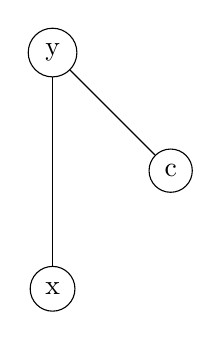
\begin{tikzpicture}
      \node[shape=circle,draw=black] (A) at (0,0) {x};
      \node[shape=circle,draw=black] (B) at (0,3) {y};
      \node[shape=circle,draw=black] (C) at (1.5,1.5) {c};

      \path [-] (A) edge node {} (B);
      \path [-] (C) edge node {} (B);
    \end{tikzpicture}
  \end{minipage}
  \begin{minipage}{0.4\linewidth}
    $\Gamma = \{ c^{y}:\tau \sepimp \upsilon, x^{y}:\tau, y^{\{c,x\}}:\tau' \}$
  \end{minipage}
  \end{framed}
  \caption{Sharing graph and typing context for $\lambda^{\sepimp} c. \lambda^{\sepimp}  x. \lambda^{\shimp}y. c x$}
  \label{fig:example-sharing-graph}
\end{figure}

The rules given in \cref{fig:bi-base-typing-rules}
are convenience rules for base cases that compute predicate constraints for types within a context.

\begin{figure}[h]\centering
  \begin{framed}
    \fbox{$P \vdash \cdot\ \texttt{un}$}
  \begin{minipage}{0.50\linewidth}
    \begin{prooftree}
      \AxiomC{$P \Rightarrow \texttt{Un}\ \tau$}\RightLabel{[\texttt{Un}-$\tau$]}
      \UnaryInfC{$P \vdash \tau\ \texttt{un}$}
    \end{prooftree}
  \end{minipage}%
  \begin{minipage}{0.50\linewidth}
    \begin{prooftree}
      \AxiomC{$P,\pi \vdash \rho\ \texttt{un}$}\RightLabel{[\texttt{Un}-$\rho$]}
      \UnaryInfC{$P \vdash \pi \Rightarrow \rho\ \texttt{un}$}
    \end{prooftree}
  \end{minipage}

  \begin{minipage}{0.50\linewidth}
    \begin{prooftree}
      \AxiomC{$P, \texttt{Un}\ t \vdash \sigma\ \texttt{un}$}\RightLabel{[\texttt{Un}-$\sigma$]}
      \UnaryInfC{$P \vdash \forall t.\sigma\ \texttt{un}$}
    \end{prooftree}
  \end{minipage}%
  \begin{minipage}{0.50\linewidth}
    \begin{prooftree}
      \AxiomC{$\bigwedge_{x:\sigma \in \Gamma}P \vdash \sigma\ \texttt{un}$}\RightLabel{[\texttt{Un}-$\Gamma$]}
      \UnaryInfC{$P \vdash \Gamma\ \texttt{un}$}
    \end{prooftree}
  \end{minipage}

  \fbox{$P \vdash \cdot \geq \cdot$}
  \begin{minipage}{0.50\linewidth}
    \begin{prooftree}
      \AxiomC{$P \Rightarrow \tau \geq \phi$}\RightLabel{[$\geq$-$\tau$]}
      \UnaryInfC{$P \vdash \tau \geq \phi$}
    \end{prooftree}
  \end{minipage}%
  \begin{minipage}{0.50\linewidth}
    \begin{prooftree}
      \AxiomC{$P,\pi \vdash \rho \geq \phi$}\RightLabel{[$\geq$-$\rho$]}
      \UnaryInfC{$P \vdash (\pi \Rightarrow \rho) \geq \phi$}
    \end{prooftree}
  \end{minipage}

  \begin{minipage}{0.50\linewidth}
    \begin{prooftree}
      \AxiomC{$P, \texttt{Un}\ t \vdash \sigma \geq \phi$}\RightLabel{[$\geq$-$\sigma$]}
      \UnaryInfC{$P \vdash (\forall t.\sigma) \geq \phi$}
    \end{prooftree}
  \end{minipage}%
  \begin{minipage}{0.50\linewidth}
    \begin{prooftree}
      \AxiomC{$\bigwedge_{x:\sigma \in \Gamma}P \vdash \sigma \geq \phi$}\RightLabel{[$\geq$-$\Gamma$]}
      \UnaryInfC{$P \vdash \Gamma \geq \phi$}
    \end{prooftree}
  \end{minipage}
\end{framed}
  \caption{Entailment Rules for Base cases}
  \label{fig:bi-base-typing-rules}
\end{figure}


\section{Syntax Directed Typing rules}\label{sec:syntax-typing-rules}
Ideally the typing rules and syntactic forms should have one-to-one
correspondence. The type system explained in the \cref{sec:type-system} is not syntax directed and will not be fit
to develop a type inference algorithm. In this section we will define syntax directed typing rules
that will simplify our type inference system shown in \cref{fig:syntax-typing-rules}

We define generalization and instantiation to express introduction and elimination of polymorphism in our
syntax direct typing rules as follows:
\begin{defn}[Instantiation]
  For a type scheme $\sigma := \forall \vec{t}. P \Rightarrow \tau'$, we say $(Q \Rightarrow \tau)$ is
  an instance of $\sigma$ and write it as $(Q \Rightarrow \tau) \sqsubseteq \sigma$, if there exists a $\vec{v}$
  such that $\tau = [\vec{v} / \vec{t}] \tau'$ and $Q = [\vec{v} / \vec{t}]P$.
\end{defn}

\begin{defn}[Generalization]
  For a type assignment $\Gamma$ and qualified type $\rho$, we define type scheme
  $\texttt{Gen}(\Gamma, \rho) = \forall (\texttt{fvs}(\rho) \backslash \texttt{fvs}(\Gamma)). \rho$.
\end{defn}

\begin{defn}[Qualified Type Scheme]
  A qualified type scheme is a pair of type scheme with a set of predicates written as $(P \mid \sigma)$,
  where $\sigma = \forall \vec{t}. Q \Rightarrow \tau$.
\end{defn}
% \begin{defn}[Qualified Type Scheme Instantiation]
%   For two qualified type schemes $(P \mid \sigma)$ where $\sigma = \forall \vec{t}. Q \Rightarrow \tau$ and
%   $(P' \mid \sigma')$ where $\sigma' = \forall \vec{t'}. Q' \Rightarrow \tau'$ we say $(P' \mid \sigma')$ is an
%   instance of $(P \mid \sigma)$ iff there exists $\vec{v}$ such that $\tau' = [\vec{v}/ \vec{t}]\tau$ and
%   $P',Q' \Rightarrow P, [\vec{v}/ \vec{t}]Q$. We write it as $(P' \mid \sigma') \sqsubseteq (P \mid \sigma)$. A type scheme
%   $\sigma$ is an abbreviation of $(\emptyset \mid \sigma)$.
% \end{defn}

The elimination of polymorphism [$\forall$E] and qualified types[$\Rightarrow$E] is always done in the [Var$^s$],
introduction of polymorphism [$\forall$I] and qualified types[$\Rightarrow$I] is
done at \texttt{let} bindings [Let$^s$]. This collapses the rules [$\forall$E], [$\Rightarrow$E] and [ID] in one rule [VAR$^s$] where
we use instantiation or specialization of type variables, and [$\forall$I], [$\Rightarrow$I] and [Let] in one rule [Let$^s$] where we use generalization of type variables.
[$\sepimp$I$^s$] is used in occurence of $\lambda^{\sepimp} $, and [$\shimp$I$^s$] is used in occurence of $\lambda^{\shimp}$.
We would add the introduced abstraction variable, $x$, into the sharing context in case of [$\shimp$I$^s$].
We collapse the application rules [$\sepimp$E] and [$\shimp$E] into one rule [App$^s$] where we check for sharing of the used variables in both
the expressions and then assign a predicate of $\texttt{ShFun}$ or $\texttt{SeFun}$ depending on whether the variables
are shared or not. The \texttt{un} predicates are added to the types of the terms that are not used directly in the expression
or which are not in sharing with the terms used.

\begin{figure}[h]\centering
  \begin{framed}
    % VAR^s
    \begin{minipage}{1.0\textwidth}
      \begin{prooftree}
        \AxiomC{$P \vdash \Gamma_{\vec{y}}\ \texttt{un}$}
        \AxiomC{$(P \Rightarrow \tau) \sqsubseteq \sigma$} \RightLabel{[VAR$^s$]}
        \BinaryInfC{$P \mid \Gamma, x^{\vec{y}} : \sigma \vdashs x : \tau $}
      \end{prooftree}
    \end{minipage}
    \newline\newline\newline
    % Let^s
    \begin{minipage}{1.0\textwidth}
      \begin{prooftree}
        \AxiomC{$Q \mid (\Gamma_x' \varoplus \Gamma_x'') \circledast \Delta \vdashs M: \upsilon\ \ \ \ \
          P \vdash \Delta\ \texttt{un}$}\def\extraVskip{0pt}\noLine
        \UnaryInfC{$P \mid (\Gamma_x, x^{\emptyset}:\sigma) \varoplus \Gamma_x'' \circledast \Delta \vdashs N:\tau\ \ \ \ \
          \sigma = \texttt{Gen}(\{\Gamma' \varoplus \Gamma_x'' \circledast \Delta \}, Q \Rightarrow \upsilon)$}\def\extraVskip{2pt}\RightLabel{[Let$^s$]}
        \UnaryInfC{$P \mid (\Gamma \circledast \Gamma') \varoplus \Gamma'' \circledast \Delta \vdashs (\Let{x}{M}{N}) : \tau$}
      \end{prooftree}
    \end{minipage}
    \newline\newline\newline
    % -*>I^s
    \begin{minipage}{0.5\textwidth}
      \begin{prooftree}
        \AxiomC{$P \Rightarrow \SeFun{\phi}$}
        \AxiomC{$P \vdash \Gamma \geq \phi$}\def\extraVskip{0pt}\noLine
        \BinaryInfC{$\ \ \ \ \ \ \ P \mid \Gamma \circledast x^{\emptyset}:\tau \vdashs M: \upsilon\ \ \ \ \ \ \ $}\def\extraVskip{2pt}\RightLabel{[$\sepimp$I$^s$]}
        \UnaryInfC{$P \mid \Gamma \vdashs \lambda^{\sepimp} x. M : \phi \tau \upsilon$}
      \end{prooftree}
    \end{minipage}%
    % -&>I^s
    \begin{minipage}{0.5\textwidth}
      \begin{prooftree}
        \AxiomC{$P \Rightarrow \ShFun{\phi}\ \ \ \ \ P \vdash \Gamma \geq \phi$}\def\extraVskip{0pt}\noLine
        \UnaryInfC{$P \mid \Gamma^{[\emptyset \mapsto \{x\}]} \varoplus x^{\texttt{Vars}(\Gamma)}:\tau \vdashs M: \upsilon$}\def\extraVskip{2pt}\RightLabel{[$\shimp$I$^s$]}
        \UnaryInfC{$P \mid \Gamma \vdashs \lambda^{\shimp}x. M : \phi \tau \upsilon$}
      \end{prooftree}
    \end{minipage}
    \newline\newline\newline
    % App^s
    \begin{minipage}{1.0\textwidth}
      \begin{prooftree}
        \AxiomC{$P \mid \Gamma \circledast \Delta \vdashs M: \phi \upsilon \tau\ \ \ \ \
          P \mid  \Gamma' \circledast \Delta \vdashs N: \upsilon$}
        \AxiomC{$P \vdash \Delta\ \texttt{un}$}\def\extraVskip{0pt}\noLine
        \BinaryInfC{$(\Gamma \tightoverset{\thicksim}{\varoplus} \Gamma' \wedge (P \Rightarrow \ShFun{\phi}))
          \vee (\Gamma \tightoverset{\thicksim}{\circledast} \Gamma' \wedge (P \Rightarrow \SeFun{\phi}))$}\def\extraVskip{2pt}\RightLabel{[App$^s$]}
        \UnaryInfC{$P \mid \Gamma \sqcup \Gamma' \circledast \Delta \vdashs M N: \tau$}
      \end{prooftree}
    \end{minipage}
    \newline\newline\newline
    \fbox{Context Operations}

    \begin{minipage}{0.5\textwidth}
      \begin{flalign*}
        \Gamma \tightoverset{\thicksim}{\circledast} \Delta = \texttt{Used}(\Gamma) \mathbin{\#} \texttt{Vars}(\Delta) \wedge \texttt{Used}(\Delta) \mathbin{\#} \texttt{Vars}(\Gamma)
      \end{flalign*}
    \end{minipage}%
    \begin{minipage}{0.5\textwidth}
      \begin{flalign*}
        \Gamma \tightoverset{\thicksim}{\varoplus} \Delta = \texttt{Used}(\Gamma) = \texttt{Used}(\Delta)
      \end{flalign*}
    \end{minipage}
  \end{framed}
  \caption{Syntax Directed Typing Rules}
  \label{fig:syntax-typing-rules}
\end{figure}

The [Let$^s$] rule defines an expression within another expression locally i.e. x would
not be in scope other than its use in $N$. We partition the typing context into multiple parts.
$\Gamma$ contains the variables that exists exclusively in $M$ and $\Gamma'$ which
are exclusively in $N$. $\Gamma''$ is common to both $M$ and $N$ while $\Delta$ is not used in either expressions $M$ or $N$.
Thus $\Gamma$ and $\Gamma'$ will be completely separate from each other while $\Gamma''$ would be in sharing with both $\Gamma$ and $\Gamma'$.
$\Delta$ would be unrestricted as it is not being shared by either $M$ or $N$. The sharing of $x$ with $\Gamma$ would depend on
whether $\Gamma$ and $\Gamma'$ are completely disjoint or empty. For the application rule [App$^s$] the type assignment $\Gamma$ would contain
variables for $M$ and $\Gamma'$ for $N$. If they are completely separate, it would be a separating function application and $M$ would be
assigned a type $\tau' \sepimp \tau$ else, they would have to be completely sharing and $M$ would be assigned a type $\tau' \rightarrow \tau$.
The conditions outlined for [App$^s$] do not look as if they are syntax directed and in the cases where the type checker cannot directly infer if the
resources used are separate or shared, the user would be expected to provide it using type annotations. $\Gamma \tightoverset{\thicksim}{\circledast} \Delta$
is an assertion that there exists a proof either possible to find by inspecting the type assignment, or provided by the user
that $\Gamma \circledast \Delta$ is defined. Similarly, $\Gamma \tightoverset{\thicksim}{\varoplus} \Delta$ means that $\Gamma \varoplus \Delta$ is well
defined.

We now state two important theorems regarding the type system and the syntax directed type system. The proofs of both the
theorems are given in \cref{chp:proofs}.

\begin{theorem}[Soundness of $\vdash^s$]
  If $P \mid \Gamma \vdash^s M:\tau$ then $P \mid \Gamma \vdash M : \tau$
\end{theorem}
The soundness property captures the essence that derivations in the syntax directed type system follow the original type system.

\begin{theorem}[Completeness of $\vdashs$]\label{thm:completeness-syntax-directed}
  If $P \mid \Gamma \vdash M:\sigma$ then
  $\exists Q, \tau$ such that $Q \mid \Gamma \vdashs M:\tau$
  and $(P \mid \sigma) \sqsubseteq \texttt{Gen}(\Gamma, Q \Rightarrow \tau)$
\end{theorem}

The completeness theorem states that we can always find predicates $Q$ and a suitable type $\tau$ for the term $M$ under the assumptions
$\Gamma$ using syntax directed type system if the original type system asserts that the typing judgement indeed exists.

\section{Type Inference and Algorithm $\M$}\label{sec:algorithm-m}
We now describe the type inference algorithm based on the previously defined syntax directed
type system. We use a variation of algorithm $\M$ \citep{lee_proofs_1998} for type inference.
We address three independent concerns in the type inference algorithm.
The first being treatment of polymorphism to be same as Hindley-Milner style. The second, we introduce
\texttt{Un} predicates for types that are unrestricted. We track this with the help of carrying a
collection of used variables throughout the algorithm which detects whether a variable is discarded
or used multiple types. The third being accounting for sharing of the variables.
The complete algorithm is outlined in \cref{fig:algorithm-m}. The input to the algorithm includes the term $M$ whose
type has to be inferred, $\tau$ is the expected type of the term, $S$ is the current substition and the
sharing information $\Psi$. The output includes the set of new predicates $P$ that are generated,
the new set of substitutions $S'$, the used variables $\Sigma$, and the new sharing information $\Psi'$.
The type variables $u$ with a subscript denote fresh variables.

We define some auxilary functions in \cref{fig:aux-defs} to lift predicates into the type system.
$Leq(\phi, \Gamma)$ adds the predicate $\phi \geq \sigma$ for all $\sigma$ that are in $\Gamma$.
$\texttt{Weaken}(x, \sigma, \Sigma, \Psi)$ adds the unrestricted predicate to the type $\sigma$
if $x$ does not belong to $\Sigma$. $\texttt{Un}(\Gamma)$ adds an unrestricted
predicate to all the types of the variables that are in the domain of $\Gamma$.
$\texttt{GenI}(\Gamma, P \Rightarrow \tau)$ generalizes the qualified type to a type scheme.
$\mathcal{C}(\Gamma, \Psi, \Sigma)$ computes the sharing information of variables in $\Gamma$
restricted to the variables in $\Sigma$.

\begin{figure}[h]
  \begin{framed}
    \begin{minipage}{0.5\linewidth}
      \begin{flalign*}
        Leq(\phi, \Gamma)  = \bigcup_{(x:\sigma) \in \Gamma} \{P \mid P \vdash \sigma \geq \phi \}
      \end{flalign*}
    \end{minipage}%
    \begin{minipage}{0.5\linewidth}
      \begin{flalign*}
        \texttt{Un}(\Gamma)  = \bigcup_{(y:\sigma) \in \Gamma}\{P \mid P \vdash \sigma\ \texttt{un} \}
      \end{flalign*}
    \end{minipage}
    \newline\newline
    \begin{minipage}{0.5\linewidth}
      \begin{flalign*}
        \texttt{GenI}(\Gamma, P &\Rightarrow \tau)  = \\
        &\forall (\texttt{fvs}(P) \cup \texttt{fvs}(\tau) \backslash\texttt{fvs}(\Gamma))). P \Rightarrow \tau
      \end{flalign*}
    \end{minipage}%
    \begin{minipage}{0.5\linewidth}
      \begin{flalign*}
        \mathcal{C}(\Gamma, \Psi, \Sigma)  = \bigcup_{x \in \texttt{dom}(\Gamma) \wedge x \in \Sigma} \Psi(x)
      \end{flalign*}
    \end{minipage}
    \newline\newline
    \begin{minipage}{1\linewidth}
      \begin{flalign*}
        \texttt{Weaken}(x, \sigma, \Sigma, \Psi)  = \begin{cases}
          P\ \ \ \ &\text{if}\ x \notin \Sigma \wedge \Psi(x) \mathbin{\#} \Sigma, P \vdash \sigma\ \texttt{un}\\
          \emptyset\ \ \ &otherwise
        \end{cases}
      \end{flalign*}
    \end{minipage}
  \end{framed}
  \caption{Auxiliary Functions}
  \label{fig:aux-defs}
\end{figure}

\begin{figure}[h]
  \begin{framed}
    {\small
      \begin{minipage}[ht]{1\linewidth}
        \centering
        \fbox{
          $\M(S, \Psi, \Gamma \vdash M : \tau) = P, S', \Sigma, \Psi'$
        }
      \end{minipage}
      % x var
      \begin{minipage}{1\linewidth}
        \begin{flalign*}
          \M(S, \Psi, \Gamma \vdash x : \tau) &= ([\vec{u} / \vec{t}]P), S' \circ S, \{x\}, \Psi \\
          \text{where\qquad}\ (x : \forall \vec{t}. P \Rightarrow \upsilon) &\in S \Gamma \\
          S' &= \Unf([\vec{u} / \vec{t}]\upsilon, S \tau)
        \end{flalign*}
      \end{minipage}

      % \&x. M: t
      \begin{minipage}{1\linewidth}
        \begin{flalign*}
          \M(S, \Psi, \Gamma \vdash \lambda^{\shimp} x. M : \tau) &= \{P \cup Q \}, S', \Sigma \backslash x, \Psi''  \\
          \text{where\qquad}\ P; S'; \Sigma; \Psi' &= \M(\Unf(\tau, u_1 u_2 u_3) \circ S, \Psi, \Gamma, x:u_2 \vdash M: u_3) \\
          Q &= \{\ShFun{u_1}\} \cup \texttt{Leq}(u_1, \Gamma|_{\Sigma}) \cup \texttt{Weaken}(x, u_2, \Sigma)\\
          \Psi'' &= \{\forall_{y \in \texttt{dom}(\Psi')}. \Psi'(y) + x\} \cup \{(x, \{ y \mid y \in \texttt{dom}(\Gamma) \})\}
        \end{flalign*}
      \end{minipage}

      % \*x. M: t
      \begin{minipage}{1\linewidth}
        \begin{flalign*}
          \M(S, \Psi, \Gamma \vdash \lambda^{\sepimp}  x. M : \tau) &= \{ P \cup Q \}, S', \Sigma \backslash x, \Psi''\\
          \text{where\qquad}\ P; S'; \Sigma; \Psi' &= \M(\Unf(\tau, u_1 u_2 u_3) \circ S, X; \Gamma, x:u_2 \vdash M: u_3) \\
          Q &= \{\SeFun{u_1}\} \cup \texttt{Leq}(u_1, \Gamma\mid_{\Sigma}) \cup \texttt{Weaken}(x, u_2, \Sigma)\\
          \Psi'' &= \Psi' \cup \{(x, \{ x \})\}
        \end{flalign*}
      \end{minipage}

      % M N: t
      \begin{minipage}{1\linewidth}
        \begin{flalign*}
          \M(S, \Psi, \Gamma \vdash M N : \tau) &= \{ P \cup P' \cup Q \}, R', \Sigma \cup \Sigma', \Psi'' \\
          \text{where\qquad}\ P; R; \Sigma; \Psi' &= \M(S, \Psi, \Gamma \vdash M:  u_1 u_2 \tau) \\
          P'; R'; \Sigma'; \Psi'' &= \M(S R, \Psi', S \Gamma \vdash N: u_2)\\
          \text{if}\ \mathcal{C}(\Gamma, \Psi'', \Sigma) &= \mathcal{C}(\Gamma, \Psi'', \Sigma')\\
          \text{then}\ Q &= \{\ShFun{u_1}\} \\
          \text{else}\ \text{if}\ &(\Sigma \# \mathcal{C}(R\Gamma, \Psi'', \Sigma')\ \text{and}\ \Sigma' \# \mathcal{C}(R\Gamma, \Psi'', \Sigma))\\
          &\text{then}\ Q = \{\SeFun{u_1}\}
          %\text{else}\ Q &= \{\SeFun{u_1}\} \cup \text{Un}(\Gamma|_{\Sigma \cap \Sigma'})
        \end{flalign*}
      \end{minipage}

      % let x = M in N: t
      \begin{minipage}{1\linewidth}
        \begin{flalign*}
          \M(S, \Psi, \Gamma \vdash \Let{x}{M}{N} : \tau) &= (P \cup Q), R', \Sigma \cup \{\Sigma' \backslash x \}, \Psi'' \\
          \text{where\qquad}\ P; R; \Sigma; \Psi' &= \M(S, \Psi, \Gamma \vdash M:u_1)  \\
          \sigma &= \texttt{GenI}(R\Gamma; R(P \Rightarrow u_1)) \\
          P'; R'; \Sigma'; \Psi'' &= \M(R, \Psi', \Gamma, x:\sigma \vdash N : \tau) \\
          Q &= \texttt{Un}(\Gamma|_{\Sigma \cap \Sigma'}) \cup \texttt{Weaken}(x, \sigma, \Sigma')
        \end{flalign*}
      \end{minipage}
    }
  \end{framed}
  \caption{Type Inference Algorithm $\mathcal{M}$}
  \label{fig:algorithm-m}
\end{figure}

% Explain each case of algorithm M here.

% Var
The first case in algorithm $\M$ in \cref{fig:algorithm-m} describes the variable case, where we are given the variable identifier and
the expected type. We try to unify the expected type $\tau$ with the derived type scheme
$\nu$ from the type assignment $\Gamma$. The return values of the algorithm are
a new set of predicates which are nothing but instantiated version of the predicates
obtained from the typing scheme, the variable $x$ being used and the new
substitution which is combination of the unification algorithms output and the original
substitution. There is no change in the sharing information and $\Psi$ is returned as is.

% \&x
In next case of sharing function introduction rule $\lambda^{\shimp}x.M$, as per the [$\shimp$I] rules, the entitites returned
are union of four predicate categories. The first is assigning a the predicate of the function to be
a sharing function $\ShFun{u_1}$, where $u_1$ is a new type variable for the type of function argument $x$.
The second assigning the function to be less restricting than the other variables in the typing assignment $\Gamma$.
The third, assigning an unrestricted predicate to the binding variable $x$ if it has not been used
anywhere in the lambda body $M$, which is done by the $\texttt{Weaken}$ function and the fourth
being the predicates generated by recursively type checking the body of the lambda expression $M$.
We create sharing links for $x$ with all the variables within the typing context $\Gamma$ in updated
$\Psi''$.
% \*x
The case of separating function $\lambda^{\sepimp} x. M$ is very similar to the previous case of $\lambda^{\shimp}x. M$ except
the that there is no sharing information to be updated as the argument to the function is
separate from its body and the function predicate assigned is $\SeFun{u_1}$ to denote this very
separating relation instead of $\ShFun u_1$

% App
In the application case the algorithm typechecks the subexpressions $M$ as a function type having
an input of the type of $N$. The additional check done here is to identify whether $M$ has a sharing
application or a separating application. If all the variables used in $M$ are also used in $N$ then
it is a sharing application i.e. $M$ is assigned a sharing function predicate $\ShFun{}$
else if the used variables in $M$ are disjoint to the variables that
are shared by $N$ or if the variables shared by variables in $M$ are disjoint to the variables
that are used in $N$, $M$ is assigned the predicate type $\SeFun{}$. Incase of a separating function
application, the variables that are used in both are marked as unrestricted. This is captured by
$\texttt{Un}(\Gamma|_{\Sigma \cap \Sigma'})$ where $\Gamma|_{\Sigma}$ means the typing assignment $\Gamma$
restricted to the variables in $\Sigma$.
% Let
In the polymorphic \texttt{let} case we first check for the type of the expression $M$ and
ensure that the variable binding $x$ is not usd in it to avoid recursive definition which would
lead to infinite types. We then generalize the computed type to $\sigma$ and then check the type of expression $N$
by expanding the type assignment $\Gamma$ with the variable $x$ and type scheme $\sigma$.

We now state the soundness theorem for the algorithm $\M$.
\begin{theorem}[Soundness of $\M$]
  if $\M(S, \Psi, \Gamma \vdash M : \tau) = P, S', \Sigma, \Psi'$ then $S' P \mid S' (\Gamma |_\Sigma ) \vdash M : S' \tau$
\end{theorem}
The soundness theorem for algorithm $\M$ ensures that the type inference algorithm inferes a type that the original type system would have
produced. The proof is given in \cref{chp:proofs}.

This type inference algorithm is however not complete. There would be cases where a term can be typed in two ways.
Algorithm $\M$ would compute only one of them and leave out the other one. Consider the type for $\lambda^{\sepimp}f. \lambda^{\sepimp}x. f x x$.
This term can be inferred to have two types by using algorithm $\M$.
\begin{itemize}
  \item $\texttt{Un}\ A \mid \emptyset \vdash \lambda^{\sepimp}f. \lambda^{\sepimp}x. f x x: (A \sepimp A \sepimp B) \sepimp A \sepimp B$
  \item $\emptyset \mid \emptyset \vdash \vdash \lambda^{\sepimp}f. \lambda^{\sepimp}x. f x x: (A \sepimp A \shimp B) \sepimp A \shimp B$.
\end{itemize}

% We summarize the proof results in \cref{fig:proof-summary}

% \begin{figure}[h]
%   \centering
%   \fbox{$\Gamma \vdash M:\tau$} \fbox{$\Gamma \vdashs M:\tau$} \fbox{$\M(\Gamma \vdash M:\tau)$}
%   \caption{Proof Summary}
%   \label{fig:proof-summary}
% \end{figure}


%%% Local Variables:
%%% mode: latex
%%% TeX-master: "../thesis-ku"
%%% End:
